\documentclass[unicode]{beamer}
\usetheme{Copenhagen}
\usepackage{luatexja,tikz}% japanese
\usetikzlibrary{cd}
\usepackage[ipaex]{luatexja-preset}% IPAex font
\usecolortheme[RGB={15,95,125}]{structure}
\usefonttheme{professionalfonts} %font of mathematical formula
\usepackage{mlmodern}%thick math font 

\title{タリラリランのコニャニャチワ}
\subtitle{tarirariran}
\author{sanbon}
\institute{chuo junior high school}
\subject{}
\begin{document}
	\begin{frame}{how to use beamer}
		\titlepage
	\end{frame}
	
	\begin{frame}{hello}
		\begin{block}{block}
			This environment is block
		\end{block}

		\begin{alertblock}{alertblock}
			This environment is alertblock
		\end{alertblock}

		\begin{exampleblock}{exampleblock}
			This environment is exampleblock
		\end{exampleblock}
	\end{frame}

	\begin{frame}{mathematical formula}
	\[ \int^\infty_{-\infty}\frac{1}{\sqrt{2\pi}}e^{-\frac{x^2}{2}} dx \]
	\end{frame}

	\begin{frame}[fragile]{tikz}
		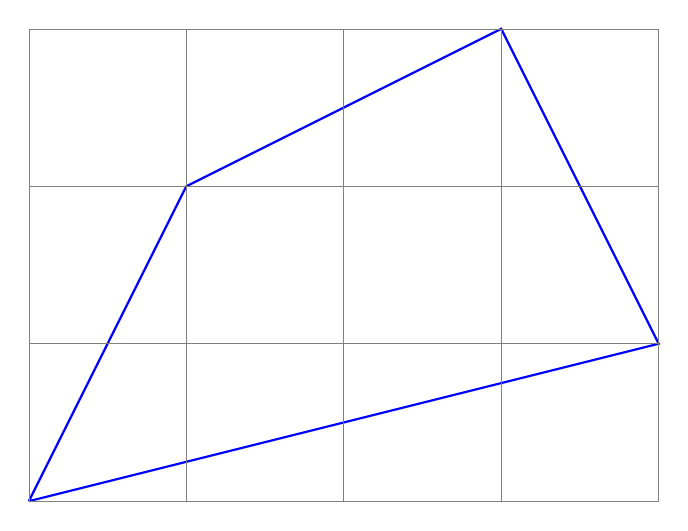
\begin{tikzpicture}[scale=2]
			\draw[color=blue,thick] (0,0) -- (1,2) -- (3,3) -- (4,1) -- (0,0);
			\draw[help lines] (0,0) grid (4,3);
		\end{tikzpicture}
		
	\end{frame}


	\begin{frame}[fragile]{commutative diagram}%fragile option kills error when you use tikz with beamer
		\[
			\begin{tikzcd}
				A \arrow[r,dash] & B \arrow[r,equal] & C \arrow[r,dotted] & D \arrow[r,dashed] & E
			\end{tikzcd}
		\]

		\[ 
			\begin{tikzcd}
			A\arrow[r,bend left=50,""{name=F,below}]\arrow[r,bend right=50,"" name=G]\arrow[Rightarrow,from=F,to=G,"\alpha"] & B
		\end{tikzcd}
	\]
	\end{frame}
\end{document}
